\documentclass[12pt]{article}
\usepackage[utf8]{inputenc}
\usepackage{graphicx}
\usepackage[a4paper,width=150mm,top=25mm,bottom=25mm]{geometry}

\title{

\\
{COS 301 SRS}
}



\author{Ctrl Alt Defeat}

\begin{document}

\begin{titlepage}
    \centering



    \vspace{2cm}
    \hrulefill\\
    \vspace{1cm}
    {\Huge\bfseries SRS Documentation v3.0}

    \vspace{1cm}

    {\Large Software Requirements Specification Document for\\Domain Pulse}\\
    \vspace{1cm}
    \hrulefill\\

    \vfill

    {\large Ctrl Alt Defeat}

    \vspace{1cm}

    {\large 2023/07/31}\\
    %    \vspace{1cm}
    %    \vspace{1cm}
    %    
\includegraphics[width=10cm]{../../Images/dpLogo.png}
    %    \vspace{1cm}\\
    %    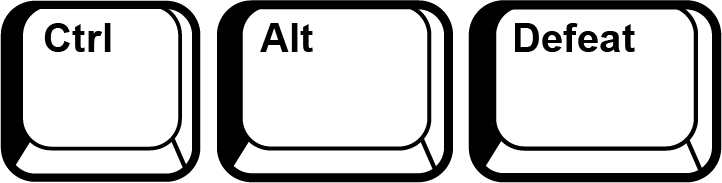
\includegraphics[width=6cm]{../../Images/cadLogo.png}

\end{titlepage}



\tableofcontents

\newpage

\section{Introduction}

\subsection{Overview}

Introducing Domain Pulse, the ultimate sentiment analysis platform. With Domain Pulse, you can easily gauge the sentiment surrounding any domain. Whether it's a business, a person, or anything else, Domain Pulse gathers information from across the internet and analyzes what people are saying.
\\\\Domain Pulse presents the results in a visually stunning and easy-to-understand format. Our wide range of visualizations brings statistics to life, making it a breeze to grasp the online presence and sentiment for any domain. Take control of understanding public opinion like never before with Domain Pulse.

\subsection{Objectives}

The objectives of the Domain Pulse project are to develop a comprehensive web application that enables users to track and analyze data from multiple sources, perform sentiment analysis, and visualize statistics. The application aims to provide a user-centered design approach, ensuring usability, accessibility, and a clear and intuitive interface. The system will be built using a scalable and modifiable architecture, leveraging microservices to handle high traffic and enable easy modification and extension. Security will be a top priority, with encryption and access control measures in place to protect user data. The project also aims to achieve high performance through caching and database optimization techniques. Overall, the objective is to create a reliable and efficient platform that empowers users to gain valuable insights from data analysis.

\newpage

\section{User Characteristics}

\newpage

\section{User Stories}

\newpage

\section{Functional Requirements}

\newpage

\section{Service Contract}

\newpage

\section{Contract Design}

\newpage

\section{Database Design}

\newpage

\section{Class Diagram}

\newpage

\section{Architectural Requirements}

\newpage

\section{Quality Requirements}

\newpage

\section{Architectural Patterns and Tactics}

\newpage

\section{Design Patterns}

\newpage

\section{Constraints}

\newpage

\section{Technology Requirements}

\newpage



\end{document}
